\documentclass[12pt, a4paper, twoside]{article}
\usepackage{fancyhdr}
\pagestyle{fancy}
\fancyhf{}
\renewcommand{\headrulewidth}{0pt}
\addtolength{\headwidth}{\marginparsep}
\addtolength{\headwidth}{\marginparwidth}
\rhead[]{\large\textbf{EXD}}
\usepackage{fontspec}
\setmainfont{Times New Roman}
\usepackage[margin=2.5cm]{geometry}
\usepackage{amsmath,amsfonts,amsthm}
\usepackage{graphicx}
% \graphicspath{{../pdfbox/}}
%% bibliography setting nature style, footnotesize in bibliography and
%% avoiding in in articles
\usepackage[style=nature,defernumbers=true,maxnames=1,firstinits=true,uniquename=init,backend=bibtex8,arxiv=abs,mcite]{biblatex}
\bibliography{../biblio}
%\renewcommand{\bibfont}{\normalfont\footnotesize}
\renewbibmacro{in:}{%
  \ifentrytype{article}{}{%
  \printtext{\bibstring{in}\intitlepunct}}}
\DeclareFieldFormat[article]{title}{}
\AtBeginBibliography{\footnotesize}
%% to set line space in bibliography
\usepackage{setspace}
%% to add affiliation to the title
\usepackage[affil-it]{authblk}
\renewcommand\Affilfont{\itshape\small}
\setlength{\affilsep}{.2em}
%% for figure caption
\usepackage[format=plain, font=scriptsize,labelfont=bf]{caption}
%% for figure wrapping
\usepackage{wrapfig}
%% for reference in a multi col
\usepackage{multicol}
% \captionsetup[figure]{font={footnotesize, stretch=1.}, belowskip=.01pt,
%   aboveskip=0.3pt}
\captionsetup[figure]{font={footnotesize, stretch=1.}, skip=0pt}
%% titling
\makeatletter
\renewcommand{\maketitle}{\bgroup\setlength{\parindent}{0pt}
\begin{flushleft}
{\LARGE
  \textbf{\@title}}

\vspace{0.3ex}

  \@author
\end{flushleft}\egroup
}
\makeatother
\title{SOL profile and fluctuations in different divertor recycling conditions in H-Mode plasmas: a cross-machine comparison}
\author{N. Vianello$^{1}$, N. Walkden$^{2}$, M. Dunne$^{2}$, B. Lomanowski$^{4}$,
  W. Wolfrum$^3$, C. Tsui$^{5, 6}$, M. Griener$^3$, D. Refy$^7$, B. Tal$^3$,  I. Cziegler$^8$, D Brida$^2$,
  O. Fevrier$^5$, H. Reimerdes$^5$, C. Theiler$^5$, M. Bernert$^2$, A. Hakkola$^9$, A. Huber$^{10}$,
  D. Carralero$^{11}$,
  V. Naulin$^{12}$,
  M. Agostini$^{1}$, J. Boedo${^6}$,
  B. Labit$^{5}$,
  H. De Oliveira$^{5}$, S. Aleiferis, I. Carvalho$^2$, C. Giroud$^2$  the ASDEX-Upgrade Team,
  the TCV-Team, the EUROfusion MST1 Team$^{*}$, and JET Contributors$^{**}$}

\affil{
  $^1$Consorzio RFX, Padova,Italy,
  $^{2}$CCFE, Culham, UK,
  $^{3}$Max-Planck-Institut f{\"u}r Plasmaphysik, Garching, Germany,
  $^{4}$Oak Ridge National Laboratory,
  $^{5}$EPFL-SPC, Switzerland,
  $^6$UCSD,  La Jolla, USA,
  $^7$Wigner Research Centre for Physics
  $^{8}$York Plasma Institute, University of York, UK,
  $^{9}$VTT, Espoo, Finland,
  $^{10}$Forschungszentrum Julich,
  $^{11}$CIEMAT Laboratorio Nacional de Fusi{\'o}n, Madrid, Spain,
  $^{12}$DTU,  Copenhagen, Denmark,
  $^{*}$See the author list B. Labit et al 2019 Nucl. Fusion 59 086020,
$^{**}$See the authors list E. Joffrin et al 2019 Nucl. Fusion 59 112021}
\date{\vspace{-3.5ex}}
%%% ------------------------------------------------------------
%%% BEGIN DOCUMENT
%%% ------------------------------------------------------------
\begin{document}
\maketitle
\vspace{-1.2em}
{\it \small Corresponding Author:} {nicola.vianello@igi.cnr.it}

Plasma Exhaust and Plasma Wall Interaction (PWI) are subjects of intense studies
in the context of fusion energy research for the understanding of the amount of heat
loads, tritium retention, and the lifetime of different Plasma Facing
Components. On this context in order to ensure reliability of
predictive edge modeling capability, it is mandatory to
determine the transport properties of the Scrape Off Layer (SOL) in
condition close to the operational point foreseen for ITER and future
devices. From the ITER divertor perspective, to
keep the power fluxes densities acceptable for target material,
high neutral pressure and partial detachment are needed to
ensure maximum tolerable loads based on avoidance of W
recrystallization \cite{pitts:2019}.
\begin{wrapfigure}[15]{l}{100mm}
%\begin{figure}[!t]
%\centering
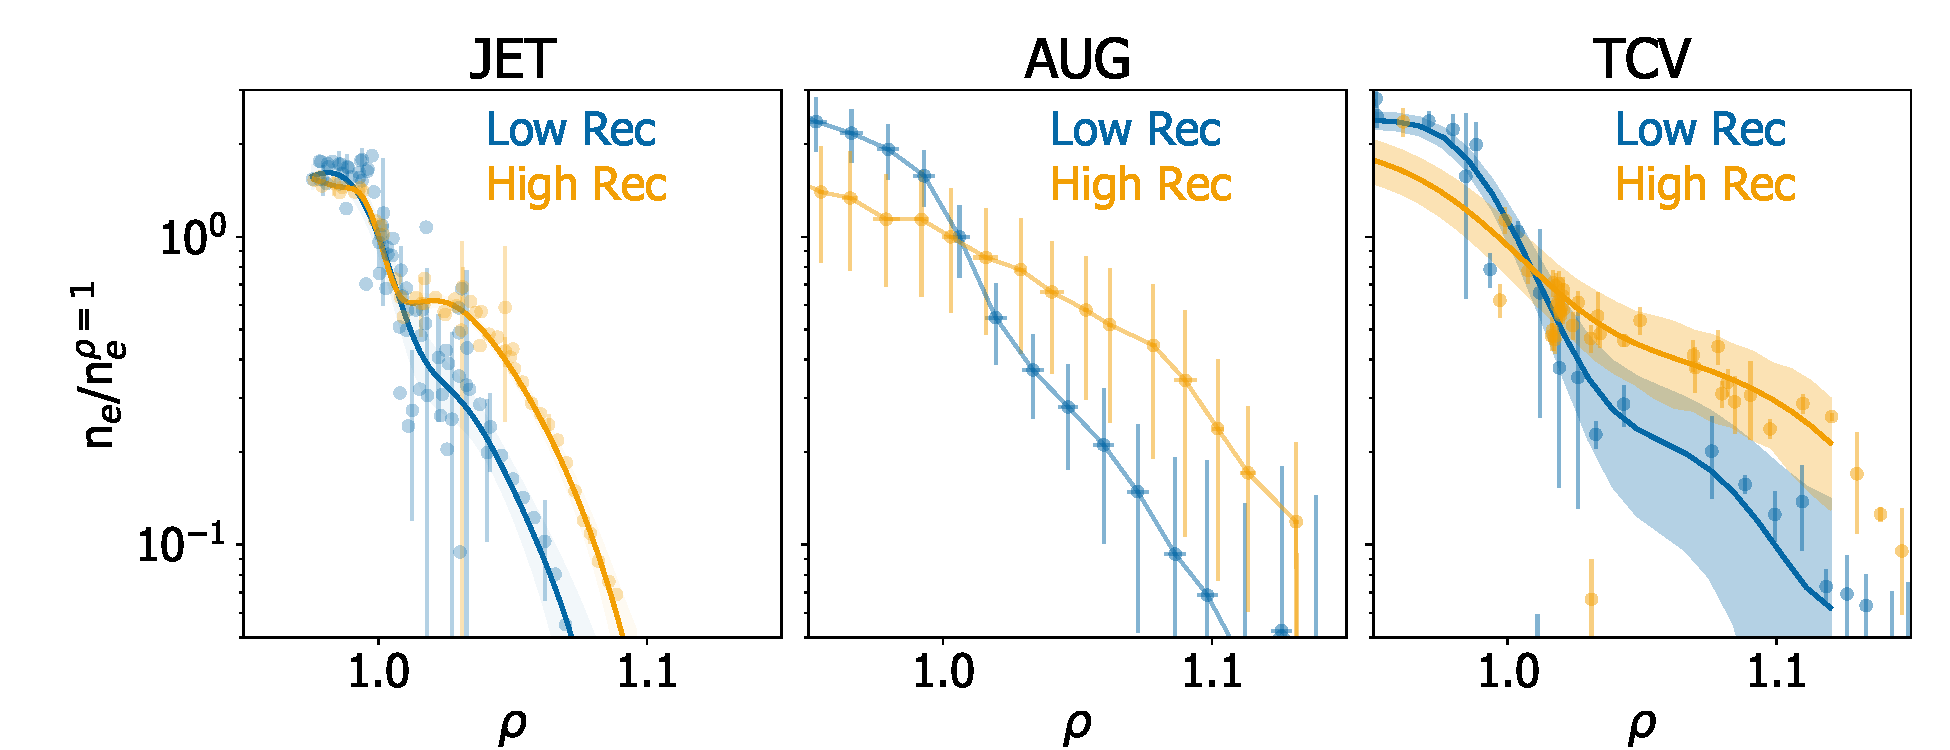
\includegraphics[width=100mm]{../pdfbox/AllUpstreamProfiles_synopsis.pdf}
\caption{Upstream profiles, normalized with
  respect to values at the separatrix in different recycling conditions.(a): JET profiles, from Li-Be and
  HRTS data superposed to a Gaussian Process Regression fit. (b) AUG, profiles gathered using Li-Be diagnostic. (c)
  TCV, where symbols representes raw data as obtained combining Thomson
 Scatering and reciprocating probe whereas the solid line represent a
 Gaussian Process Regression fit}
%\vspace{-2.6ex}
\label{fig:figProfile}
\end{wrapfigure}
Thus experimental investigation
of SOL transport needs to be extended also to these operational regimes.
The SOL properties results from a competition between sources and losses parallel and
perpendicular to the magnetic field: it is strongly dominated by
the presence of turbulent filaments, which contribute to
particle and energy losses both in L- and H-mode regimes.
In present experiments the regimes matching ITER divertor operational point are obtained
with high gas throughput leading to high density regimes. In L-Mode
these operational conditions are associated to the appearance of a
\emph{density shoulder}
i.e. progressive flattening of the density
scrape off layer profile at high density
\cite{Asakura:1997is,LaBombard:2001ks,
  Carralero:2017gb}. It has been proved that density shoulder appear
starting from high-recycling regimes and become broader after target
density rollover \cite{vianello:nf2019}, even
though differences have been observed depending on divertor geometry
\cite{Wynn:2018gp}, or if high recycling condition are achieved
through impurity seeding rather than high fuelling
\cite{Wynn:2018gp,Kuang:2019248}.
The density shoulder is actually accompained by
an increase of the filamentary activity
\cite{Carralero:2017gb,vianello:nf2019,Kuang:2019248}, together with an increase of
their associated convective transport \cite{Carralero:2017gb}. Preliminary investigations suggested that similar inter-ELM SOL
density profile broadening is observed in H-mode as well
\cite{Muller:2015jt,Carralero:2017gb,vianello:nf2019}, with a stronger
dependence on the neutral pressure \cite{vianello:nf2019}.
Furthermore
in case of highly dissipative divertor with high gas throughput the
pedestal profile modification move the plasma towards a small-ELM
regime \cite{labit:nf2019} where a clear increase of
the SOL density decay length is observed.
Despite the
large experimental effort, a comprehensive understanding
of the mechanism leading to an H-mode shoulder formation is presently
lacking and this motivated a joint experimental effort within
Eurofusion framework.
The present contribution will report results obtained in a
coordinated effort within 3 different devices, JET, ASDEX-Upgrade (AUG) and
TCV focusing on the SOL profile evolution in different divertor recycling
states, correlating the observed profile modification with different turbulent SOL
plasma transport.
\begin{wrapfigure}[12]{l}{100mm}
%\begin{figure}[!t]
%\centering
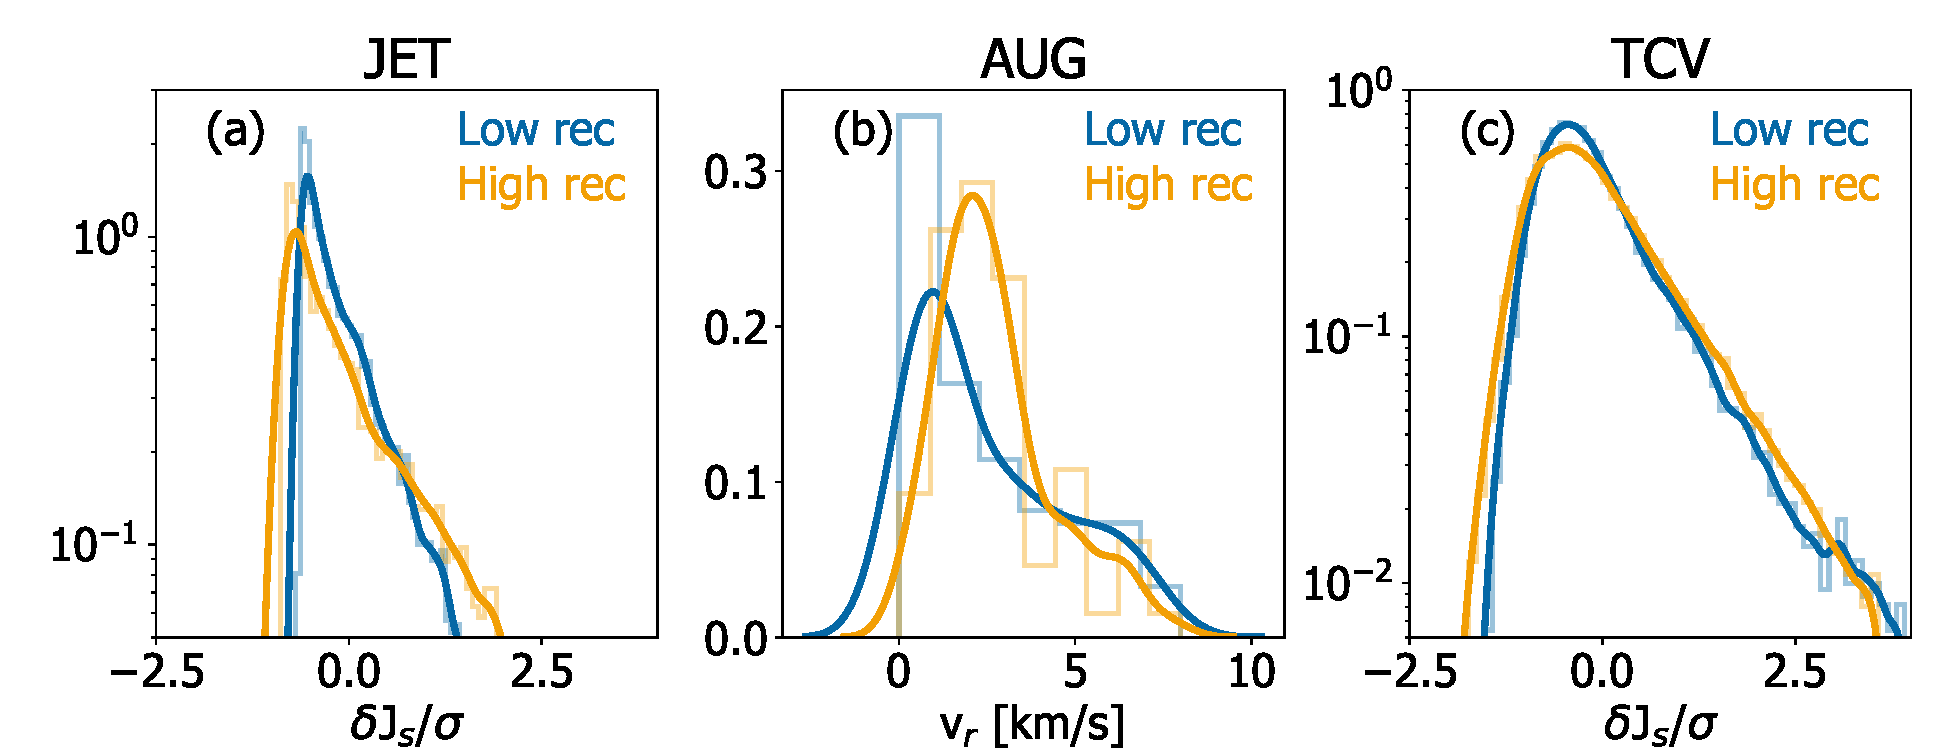
\includegraphics[width=100mm]{../pdfbox/SynopsisFluctuationCombined.pdf}
\caption{Fluctuation properties in different recycling states for the
  3 devices:(a) PDF of Jsat fluctuations at the wall on JET (b)
  inter-ELM filament velocity in the far SOL from THB diagnostic (c) PDF of Jsat fluctuations at the wall on TCV}
\vspace{-2.6ex}
\label{fig:figFluctuations}
\end{wrapfigure}

In JET, 2MA/2.3T low-$\delta$ plasma with 16 MW of
applied NBI power were analyzed, with different level of fueling both
exploring different divertor shapes
in order to tackle the dependence of different neutral compression as well
\cite{Tamain:2015cx}.
On AUG 0.8MA/2.1T scenarios at different power levels (from 3 to 17 MW) and different fuelling
schemes were analyzed in order to explore a wide range of divertor
parameters and recycling state.
Finally on TCV high-$\delta$ low current (0.18 MA)
discharges were investigated with an additional 1 MW of NBI heating
where different fueling levels and fueling schemes (main chamber or
divertor fuelling) were used. In all the devices we have been able to
identify conditions where inter-ELM density profiles at different recycling states exhibit a clear profile broadening as shown in
figure \ref{fig:figProfile}. In order to access possible contribution of SOL
turbulence induced convective transport in modifying SOL profile,
fluctuation in the main SOL and at the wall have been investigated
using different diagnostics in the various machine as shown in
\ref{fig:figFluctuations}. For AUG,  filaments velocities of
inter-ELM filaments have been determined using the Thermal Helium Beam
diagnostic \cite{Griener:20183cf} and compared with the fluctuation
observed in high-recycling state during the small-ELM regime. The
comparison of the distribution function of these velocity is shown in
\ref{fig:figFluctuations} (b) and a clear increase of the filament velocity
during high recycling state is observed. For TCV and JET we show the
Probability Distribution Function (PDF) of the ion saturation current
density J$_s$ as measured at the wall by mean of embedded langmuir
probe respectively in panels (a) and (c) of figgure
\ref{fig:figFluctuations}.
Clearly in high density/high recycling state more skewed PDF are
observed for both the machines suggesting an increase of the
fluctuation induced convective transport towards the first wall.
The contribution will provide a complete characterization of the
explored conditions in all the 3 devices in terms of divertor properties, upstream
profiles, SOL fluctuation and pedestal evolution in order to improve
the understanding of SOL transport in ITER divertor relevant
condition.

\begingroup
\setstretch{0.8}
{\footnotesize\textbf{Acknowledgment}\\
This work has been carried out within the framework of the EUROfusion Consortium and has received funding from the Euratom research and training programme 2014 - 2018 and 2019 - 2020 under grant agreement No 633053. The views and opinions expressed herein do not necessarily reflect those of the European Commission.}
\begin{multicols}{2}
\setlength\bibitemsep{0pt}
\printbibliography[heading=none]
\end{multicols}
\endgroup

\end{document}

% \begin{wrapfigure}[10]{l}{100mm}
% \centering
% 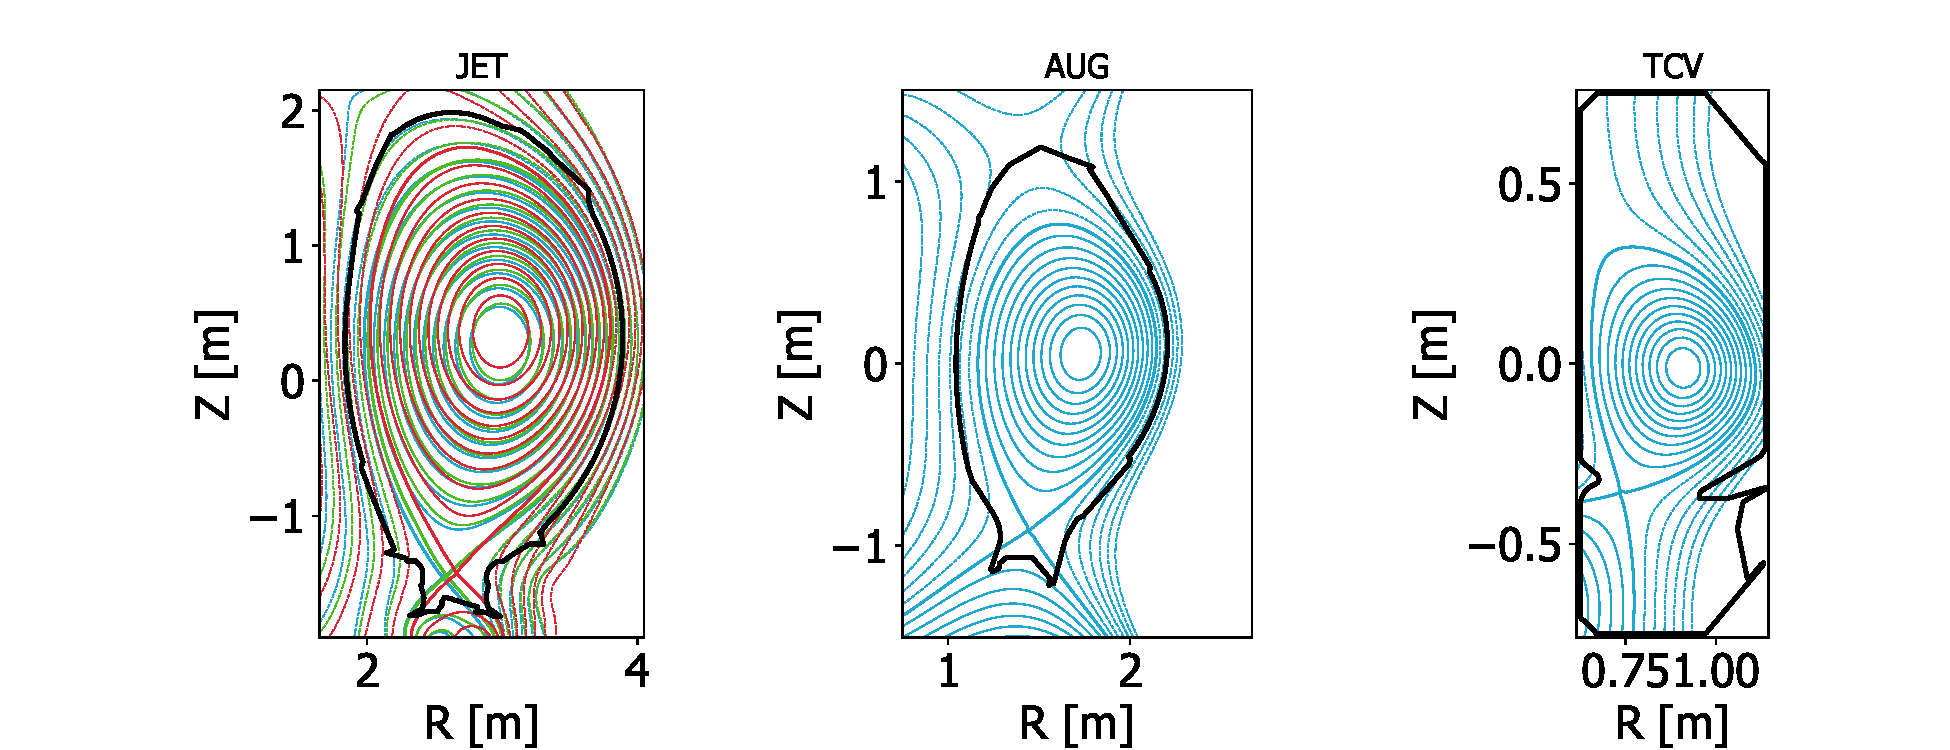
\includegraphics[width=100mm]{../pdfbox/AllEquilibria.pdf}
% \caption{Plasma shapes investigated in all the three devices. For JET
%   the 3 different configuration are shown as well}
% \vspace{-2.6ex}
% \label{fig:figEquilibria}
% \end{wrapfigure}
